\documentclass[10pt]{article}
\usepackage[a4paper,margin=18mm]{geometry}
\usepackage{graphicx,hyperref,amsmath,booktabs}
\hypersetup{colorlinks=true,urlcolor=blue}\setlength{\parindent}{0pt}\setlength{\parskip}{6pt}
\begin{document}
\begin{center}\Large Public-system root control for sparse elimination\\[3pt]
\normalsize Curve25519 native v1 --- unsigned producer evidence --- 16 November 2026\end{center}
The new isolated Rust solver returns a 71-variable witness satisfying 81
original equations and independent indexed-row/group replay:
$+\operatorname{column}(1,0)+\operatorname{column}(2,0)$.
Only public System/limits enter the query. Native PCC-20261116-9dda07.
[pcc:unverified]

\textbf{Exact scope.} The control is over $p=2^{255}-19$, on the existing
curve, with $h_{\rm new}=h_{\rm old}^{213156431}$, $q=1$, $k=2$, arity 2.
It is a TWO-column family, not the huge original base or a DLP solve.
No planted labels, signs, scalar, point list or witness enters the solver.

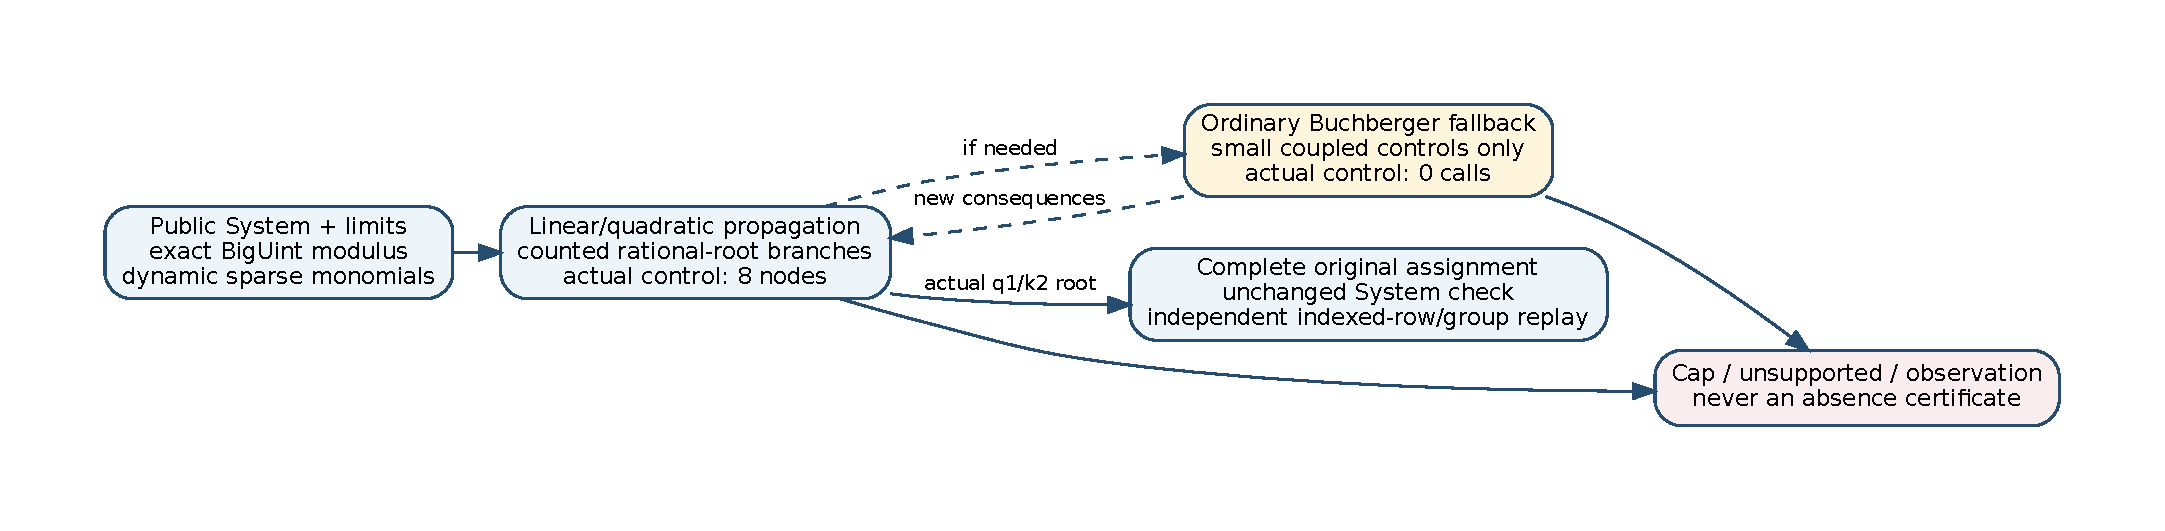
\includegraphics[width=\linewidth]{pipeline.pdf}

\textbf{Which algorithm ran.}
The actual root uses 8 propagation branches, 0 Buchberger calls and 0 S-pairs.
It demonstrates linear/quadratic propagation, not a Gr\"obner advantage or a
general degree 2 solving bound. Two small coupled quadratic controls exercise
the ordinary sparse Buchberger fallback over 101 and the actual prime.
The implementation is not matrix F4. Higher-degree extraction is explicitly
unsupported; a unit-ideal observation is not an absence certificate.

\begin{center}\begin{tabular}{p{.31\linewidth}p{.60\linewidth}}\toprule
Fixed control & Observed scope\\\midrule
Actual public relation &71 variables, 81 equations, 243 terms; original root/row replay\\
Dynamic index/width &1,100 declared variables,ONE constrained variable; large coefficient retained\\
Square-root comparison &106 agreements: all 101 residues plus five actual-field edges\\
Forced resource limits &Nine lowered caps distinguish refusal classes\\
Original six-member input &1,059 variables / 1,089 equations,FORCED work 1 refusal; no full solve attempt\\\bottomrule
\end{tabular}\end{center}

Returned roots receive original evaluation, mutation and truncated-assignment
refusal. Malformed input and noncanonical coefficient controls are retained.
These are fixed development controls, not target-yield estimates.
[pcc:unverified]

\newpage
\begin{center}\Large Counters, preservation and the next gate\end{center}
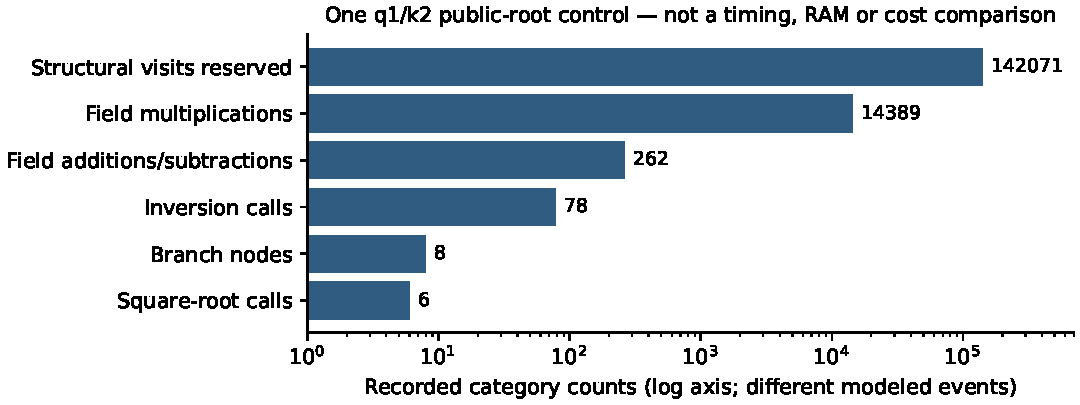
\includegraphics[width=\linewidth]{events.pdf}

\textbf{Counter scope.}
Actual-case records contain 14,389 field multiplications, 262 additions/
subtractions, 78 inversion calls, 6 square-root calls, 142,071 reserved structural
visits and 8 branch nodes. The model charges 156,814 events and cumulatively
reserves 5,251,936 represented bytes. These are not normalized GAE, elapsed time
or peak RSS. Original/group replay, parsing/serialization and full container/
allocation overhead have not been priced. Full cold-accounting acceptance
remains open. No performance ratio or attack exponent follows.
[pcc:unverified]

\textbf{Reproducibility.}
The 49-input context reuses the unchanged 43-input v2 archive plus five crate
inputs and an immutable original-system gzip. A 35,180-byte delta, six
compiled-in hashes and the retained binary qualifier match. Pre-call source/
binary hashes precede controls; complete roots, counters, stop classes and
the original 71-variable input remain beside them. Release test/fmt/strict
Clippy pass locally. Initial unused-import/source and resource-admission
audit versions remain retained. There is no independent signature or new
generic proof of field, Gr\"obner, group or compiler semantics. [pcc:unverified]

\textbf{Next discriminating work.}
Complete accounting and compare a dependency worklist against repeated
whole-system substitution on identical public equations. Then test redundant
unknown-index-bit constraints, deterministic range propagation and original
root projection. They may expose useful structure to this partial extractor;
they do not provide free indexing or a cost improvement merely by adding
labels. A matched trace compiler remains a separate comparator.

The complete route still needs useful yield, selection, relation count,
kernel, scalar replay, memory and growing-family evidence under the original
criteria. No paid job, timing, solver sampling/campaign, huge-base enumeration
or broad root-library rerun occurred.

\textbf{Sources and files.}
\href{https://people.maths.ox.ac.uk/petit/files/16PKC_primeECDLP.pdf}{Petit--Kosters--Messeng(2016), sections4/5};
\href{https://arxiv.org/abs/1503.08001}{Kosters--Yeo, Notes on summation polynomials};
immutable engine-source review PCC-20261116-3aeb9e. KB runtime unavailable;
direct primary sources were read. Classical algorithms are not claimed novel.

See \texttt{direct-elimination-v1/} protocol, qualification scope, source
manifest, native records and next gate. Old source, reports, claims, original
criteria and direct Lean bindings remain unchanged. Canonical cost graphs
are unchanged because no admitted performance datum was added.
\end{document}
